\documentclass[11pt,a4paper]{article}
\usepackage{gtu-el-yazisi}
\begin{document}
\notbilgi{Nümerik Analiz}{8. Hafta -- Nümerik İntegralleme}{Numerik-8.hafta.pdf}

\sayfa{1}
\section{Nümerik integralleme}
\noindent Belirli integraller
\[
  \int_a^b f(x)\,dx = \sum_{k=1}^{n} \alpha_k f(x_k) \qquad \text{``quadrature''}
\]
\[
  x_0, x_1, x_2, \ldots, x_n \in [a,b]
\]
Lagrange IP \qquad
$\displaystyle P_n(x) = \sum_{k=0}^{n} \underbrace{L_{n,k}(x)}_{\prod\limits_{\substack{i=0\\ i\ne k}}^{n}\frac{(x-x_i)}{(x_k-x_i)}} f(x_k)$

\medskip
$f \in C^{n+1}[a,b]$
\[
  f(x) = P_n(x) + \frac{f^{(n+1)}(\xi(x))}{(n+1)!}\prod_{i=0}^{n}(x-x_i) \qquad \xi = \xi(x) \in (a,b)
\]
\begin{align*}
  \int_a^b f(x)\,dx &= \underbrace{\int_a^b \sum_{k=0}^{n} L_{n,k}(x)\,f(x_k)\,dx}_{\text{Tahmin}}
    + \underbrace{\int_a^b \frac{f^{(n+1)}(\xi)}{(n+1)!}\prod_{i=0}^{n}(x-x_i)\,dx}_{\text{Hata}}\\
  &= \underbrace{\sum_{k=0}^{n} \alpha_k f(x_k)}_{\text{Tahmin}} + \underbrace{E(f)}_{\text{Hata}}
\end{align*}
\[
  \alpha_k = \int_a^b L_{n,k}(x)\,dx
\]

\subsection{Trapezoid (yamuk) kuralı}
\noindent
\begin{minipage}[c]{0.58\linewidth}
\begin{align*}
  f(x) \cong P_1(x) &= \frac{x-x_1}{x_0-x_1}\,f(x_0) + \frac{x-x_0}{x_1-x_0}\,f(x_1)\\
  E_1(x) &= \frac{f''(\xi(x))}{2}(x-x_0)(x-x_1) \qquad \xi \in (x_0,x_1)
\end{align*}
\end{minipage}\hfill
\begin{minipage}[c]{0.4\linewidth}
\centering
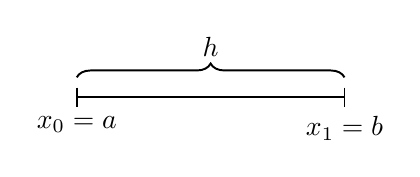
\begin{tikzpicture}[line width=0.7pt]
  \draw (0,0) -- (3.4,0);
  \draw (0,0.12) -- (0,-0.12) node[below] {$x_0 = a$};
  \draw (3.4,0.12) -- (3.4,-0.12) node[below] {$x_1 = b$};
  \draw[decorate, decoration={brace, amplitude=5pt}] (0,0.25) -- (3.4,0.25) node[midway, above=4pt] {$h$};
\end{tikzpicture}
\[
  \int_a^b f(x)\,dx = \int_a^b P_1(x)\,dx + \int_a^b E_1(x)\,dx
\]
\end{minipage}

\begin{teorem}[(İntegral için ortalama (ara) değer teoremi)]
$f \in C[a,b]$ ve $g(x)$ $a \le x \le b$ integrallenebilir ve işaretini korur
\\öyle bir $c \in (a,b)$ var ki,
\[
  \int_a^b f(x)\,g(x)\,dx = f(c)\int_a^b g(x)\,dx
\]
\end{teorem}
\begin{align*}
  &\int_{x_0}^{x_1} f''(\xi(x))\,\underbrace{(x-x_0)(x-x_1)}_{g(x)\ \text{(işaret değiştirmiyor)}}\,dx\\
  &= f''(\xi_1)\int_{x_0}^{x_1} (x-x_0)(x-x_1)\,dx \;\Bigg|_{h = x_1 - x_0} = -\frac{h^3}{6}\,f''(\xi_1)
\end{align*}

\sayfa{2}
{\small\color{kursunkalem}(Üstte karalanmış: $-\frac{h^3}{6}f''(\xi_1)$)}
\begin{align*}
  \int_a^b f(x)\,dx &= \int_a^b P_1(x)\,dx + \int_a^b E_1(x)\,dx\\
  &= \left[\frac{(x-x_1)^2}{2(x_0-x_1)}\,f(x_0) + \frac{(x-x_0)^2}{2(x_1-x_0)}\,f(x_1)\right]_{x=x_0}^{x=x_1}\\
  &\quad + -\frac{h^3}{12}\,f''(\xi_1)\\
  &= \frac{h}{2}\Big[f(x_0) + f(x_1)\Big] - \frac{h^3}{12}\,f''(\xi_1)
\end{align*}

\subsection{Simpson kuralı}
\begin{center}
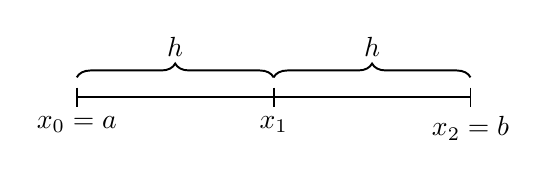
\begin{tikzpicture}[line width=0.7pt]
  \draw (0,0) -- (5,0);
  \draw (0,0.12) -- (0,-0.12) node[below] {$x_0 = a$};
  \draw (2.5,0.12) -- (2.5,-0.12) node[below] {$x_1$};
  \draw (5,0.12) -- (5,-0.12) node[below] {$x_2 = b$};
  \draw[decorate, decoration={brace, amplitude=5pt}] (0,0.25) -- (2.5,0.25) node[midway, above=4pt] {$h$};
  \draw[decorate, decoration={brace, amplitude=5pt}] (2.5,0.25) -- (5,0.25) node[midway, above=4pt] {$h$};
\end{tikzpicture}
\end{center}
\begin{align*}
  P_2(x) &= \frac{(x-x_1)(x-x_2)}{(x_0-x_1)(x_0-x_2)}\,f(x_0) + \frac{(x-x_0)(x-x_2)}{(x_1-x_0)(x_1-x_2)}\,f(x_1)\\
  &\quad + \frac{(x-x_0)(x-x_1)}{(x_2-x_0)(x_2-x_1)}\,f(x_2)
\end{align*}
\[
  \int_a^b f(x)\,dx = \int_{x_0}^{x_2} P_2(x)\,dx + \int_{x_0}^{x_1} E_2(x)\,dx
\]
{\small\color{kursunkalem}($x_1$ civarından Taylor:)}
\begin{align*}
  f(x) &= f(x_1) + f'(x_1)(x-x_1) + \frac{f''(x_1)}{2!}(x-x_1)^2 + \frac{f'''(x_1)}{3!}(x-x_1)^3\\
  &\quad + \frac{f^{(4)}(\xi)}{4!}(x-x_1)^4
\end{align*}
\begin{align*}
  \int_a^b f(x)\,dx &= \Big[f(x_1)(x-x_1) + \frac{f'(x_1)}{2}(x-x_1)^2 + \frac{f''(x_1)}{6}(x-x_1)^3\\
  &\qquad + \frac{f'''(x_1)}{24}(x-x_1)^4\Big]_{x_0}^{x=x_2}
   + \underbrace{\int_{x_0}^{x_2} \frac{f^{(4)}(\xi(x))}{24}(x-x_1)^4\,dx}_{\frac{f^{(4)}(\xi_1)}{120}\,2h^5}
\end{align*}
\[
  f''(x_1) = \frac{1}{h^2}\Big[f(x_0) - 2f(x_1) + f(x_2)\Big] - \frac{h^2}{12}\,f^{(4)}(\xi_2)
\]
\begin{align*}
  \int_a^b f(x)\,dx &= \int_{x_0}^{x_2} P_2(x)\,dx + \int_{x_0}^{x_1} E_2(x)\,dx = 2h\,f(x_1) + \ldots\\
  &\swarrow\ \frac{h^3}{3}\left[\frac{1}{h^2}\Big[f(x_0) - 2f(x_1) + f(x_2)\Big] - \frac{h^2}{12}\,f^{(4)}(\xi_2)\right]\\
  &\quad + \frac{f^{(4)}(\xi_1)\,h^5}{60}
\end{align*}

\sayfa{3}
\[
  = \frac{h}{3}\Big[f(x_0) + 4f(x_1) + f(x_2)\Big]
    - \frac{h^5}{12}\left[\frac{1}{3}\,f^{(4)}(\xi_2) - \frac{1}{5}\,f^{(4)}(\xi_1)\right]
\]
\formulkutu{\int_a^b f(x)\,dx = \underbrace{\frac{h}{3}\Big[f(x_0) + 4f(x_1) + f(x_2)\Big]}_{\text{Tahmin}}
  - \underbrace{\frac{h^5}{90}\,f^{(4)}(\xi)}_{\text{Hata}}}

\subsection{Kapalı Newton-Cotes formülü (Genelleme)}
\noindent $[a,b]$ kapalı aralık\\
\hspace*{1em}$x_0 = a$, \ $x_n = b$\\
\hspace*{1em}$x_k = x_0 + kh$ \qquad $h = \dfrac{b-a}{n}$ \qquad $k = 0, 1, \ldots, n$

\noindent
\begin{minipage}[c]{0.42\linewidth}
\centering
\begin{tikzpicture}[line width=0.7pt, xscale=0.9]
  \draw (-0.2,0) -- (5,0);
  \draw (0,-0.2) -- (0,2.4);
  \node[left] at (0,1.8) {$f(x)$};
  \draw[domain=0:4.4, samples=50, smooth] plot (\x, {1.3 + 0.5*cos(deg(\x*1.43))});
  \draw[kursunkalem, smooth] plot coordinates {(0,1.8) (0.8,1.65) (1.8,0.85) (2.8,1.05) (3.6,1.6) (4.4,1.75)};
  \draw[dashed] (3.6,0) -- (3.6,1.65);
  \foreach \x/\n in {0/x_0{=}a, 0.9/x_1, 1.8/x_2, 2.8/x_{n-1}, 3.6/x_n}{
    \draw (\x,0.08) -- (\x,-0.08) node[below, font=\small] {$\n$};}
\end{tikzpicture}
\end{minipage}\hfill
\begin{minipage}[c]{0.55\linewidth}
\[
  P_n(x) = \sum_{k=1}^{n} f(x_k)\prod_{\substack{i=0\\ i\ne k}}^{n}\frac{(x-x_i)}{(x_k-x_i)}
\]
\end{minipage}

\begin{align*}
  f(x) &= P_n(x) + \frac{f^{(n+1)}(\xi(x))}{(n+1)!}\prod_{k=0}^{n}(x-x_k)\\
  \int_a^b f(x)\,dx &\approx \int_a^b P_n(x)\,dx = \sum_{k=0}^{\infty}\footnotemark\,\alpha_k f(x_k)
\end{align*}
\footnotetext{Claude notu: muhtemelen toplamın üst sınırı $n$ olmalı.}
\[
  \alpha_k = \int_a^b \prod_{\substack{i=0\\ i\ne k}}^{n} \frac{x - x_i}{x_k - x_i}\,dx
\]

\begin{teorem}
$\displaystyle\sum_{k=0}^{n} \alpha_k f(x_k)$ \ $(n+1)$ adet noktadan \underline{kapalı NC} formülü olsun
\hfill{\small $n = 1 \rightarrow$ Trapezoid, \ $n = 2 \rightarrow$ Simpson}\\
$x_0 = a$, \ $x_n = b$ \ ve \ $h = \dfrac{b-a}{n}$\\
Böylece $\xi \in (a,b)$ sayısı, $n$ çift ve $f \in C^{n+2}[a,b]$ olacak biçimde
\[
  \int_a^b f(x)\,dx = \sum_{k=0}^{n} \alpha_k f(x_k)
  + \frac{h^{n+3}\,f^{(n+2)}(\xi)}{(n+2)!}\int_0^n t^2(t-1)\cdots(t-n)\,dt
\]
\hspace*{0.45\linewidth}$n$ tek ve $f \in C^{n+1}[a,b]$
\[
  \text{''} \qquad\qquad \text{''} \qquad
  + \frac{h^{n+1}\,f^{(n+1)}(\xi)}{(n+1)!}\int_0^n t(t-1)\cdots(t-n)\,dt
\]
formülleri \okunamadi{sağlanır}.
\end{teorem}

\sayfa{4}
\subsection{Açık Newton-Cotes formülü (Genelleme)}
\noindent $(a,b)$ açık aralık\\
\hspace*{1em}$x_{-1} = a$, \ $x_{n+1} = b$\\
\hspace*{1em}$x_k = x_0 + kh$ \qquad $h = \dfrac{b-a}{n+2}$\\
\hspace*{6em}$k = 0, 1, \ldots, n$\\[1mm]
\hspace*{1em}$\bullet$\ $x_0, x_1, \ldots, x_n \in (a,b)$
\begin{center}
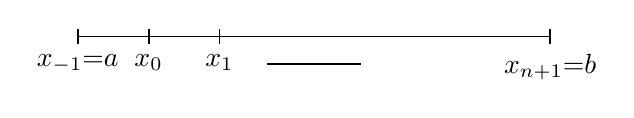
\begin{tikzpicture}[line width=0.7pt]
  \draw (0,0) -- (6,0);
  \foreach \x/\n in {0/x_{-1}{=}a, 0.9/x_0, 1.8/x_1, 6/x_{n+1}{=}b}{
    \draw (\x,0.1) -- (\x,-0.1) node[below] {$\n$};}
  \draw (2.4,-0.35) -- (3.6,-0.35);
\end{tikzpicture}
\end{center}

\noindent $n = 0$ durumunda formülü belirleyelim
\noindent
\begin{minipage}[c]{0.5\linewidth}
$h = \dfrac{b-a}{2}$ \qquad $x_0 = a + h$
\end{minipage}\hfill
\begin{minipage}[c]{0.45\linewidth}
\centering
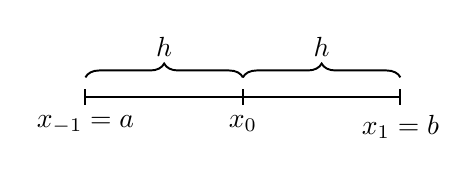
\begin{tikzpicture}[line width=0.7pt]
  \draw (0,0) -- (4,0);
  \draw (0,0.1) -- (0,-0.1) node[below] {$x_{-1} = a$};
  \draw (2,0.1) -- (2,-0.1) node[below] {$x_0$};
  \draw (4,0.1) -- (4,-0.1) node[below] {$x_1 = b$};
  \draw[decorate, decoration={brace, amplitude=5pt}] (0,0.25) -- (2,0.25) node[midway, above=4pt] {$h$};
  \draw[decorate, decoration={brace, amplitude=5pt}] (2,0.25) -- (4,0.25) node[midway, above=4pt] {$h$};
\end{tikzpicture}
\end{minipage}

\begin{align*}
  f(x) &= f(x_0) + f'(x_0)(x-x_0) + \frac{f''(\xi)}{2!}(x-x_0)^2\\
  \int_a^b f(x)\,dx &= \int_{x_{-1}}^{x_1} f(x_0)\,dx + \int_{x_{-1}}^{x_1} f'(x_0)(x-x_0)\,dx
    + \frac{1}{2}\int_{x_{-1}}^{x_1} f''(\xi(x))(x-x_0)^2\,dx\\
  &= f(x_0)(x_1 - x_{-1}) + f'(x_0)\,\frac{(x-x_0)^2}{2}\bigg|_{x_{-1}}^{x_1}
    + \frac{1}{2}\,f''(\xi_1)\int_{x_{-1}}^{x_1}(x-x_0)^2\,dx\\
  &= 2h\,f(x_0) + \frac{h^3}{3}\,f''(\xi_1)
\end{align*}
{\small\color{kursunkalem}(Son satırın başında karalanmış bir ifade var.)}

\sayfa{5}
\section{Uygulama}
\begin{ornek}
1) $\displaystyle\int_{0{,}5}^{1} x^4\,dx = \frac{31}{160} = \frac{31}{160} = 0{,}19375$ \qquad
2) $\displaystyle\int_{e}^{e+1} \frac{1}{x\ln x}\,dx \cong 0{,}2725$

İntegrallerin değerini Trapezoidal ve Simpson formülleri kullanarak tahmini hesaplayınız
\end{ornek}
\begin{cozum}
1) $f(x) = x^4$, \ $\underbrace{0{,}5}_{a} \le x \le \underbrace{1}_{b}$
\hfill $x_0 = 0{,}5$, \ $x_1 = 1$, \ $h = b - a = 1 - 0{,}5 = 0{,}5$
\begin{align*}
  \int_a^b f(x)\,dx &\approx \frac{h}{2}\Big[f(x_0) + f(x_1)\Big]\\
  \int_{0{,}5}^{1} x^4\,dx &= \frac{0{,}5}{2}\Big[(0{,}5)^4 + 1^4\Big] = \frac{1}{4}\left[\frac{1}{16} + 1\right]
     = \frac{17}{64} \approx 0{,}26
\end{align*}

\noindent{\small Simpson}
\[
  \int_a^b f(x)\,dx = \frac{h}{3}\Big[f(x_0) + 4f(x_1) + f(x_2)\Big]
  \qquad
  \begin{array}{ll}
    x_0 = 0{,}5 & x_1 = x_0 + h\\
    x_2 = 1 & h = \frac{b-a}{2}
  \end{array}
\]
\hfill $h = \dfrac{1 - 0{,}5}{2} = \dfrac{1}{4} = 0{,}25$ \qquad \fbox{$x_1 = 0{,}5 + 0{,}25 = 0{,}75$}
\begin{align*}
  \frac{1/4}{3}&\left[\left(\frac{1}{2}\right)^4 + 4\left(\frac{3}{4}\right)^4 + 1^4\right]\\
  &= \frac{1}{12}\left[\frac{1}{16} + \frac{81}{64} + 1\right] = \frac{149}{12\cdot 64} = 0{,}1940
\end{align*}

\medskip
2) \quad
$\begin{array}{ll}
  x_0 = e & x_1 = x_0 + h\\
  x_2 = e + 1 & h = \frac{b-a}{2}
\end{array}$
\begin{align*}
  h &= \frac{e + 1 - e}{2} = \frac{1}{2}\\
  x_1 &= e + \frac{1}{2} = e + 0{,}5
\end{align*}
\[
  \frac{1}{6}\left[\frac{1}{e\ln e} + 4\,\frac{1}{\left(\frac{1}{2} + e\right)\ln\left(\frac{1}{2} + e\right)}
  + \frac{1}{(1+e)\ln(1+e)}\right] \cong 0{,}2727
\]
\end{cozum}

\sayfa{6}
\begin{cozum}
$x_0 = e$, \ $x_1 = 1 + e$ \qquad $h = b - a = 1$
\[
  \int_e^{e+1} \frac{1}{x\ln x}\,dx \cong \frac{1}{2}\left[\frac{1}{e\ln e} + \frac{1}{(1+e)\ln(1+e)}\right] \cong 0{,}2863
\]
\end{cozum}

\begin{ornek}[3]
Ara nokta formülünü kullanarak
\[
  \int_0^{\pi/4} \sin x\,dx = 1 - \frac{1}{\sqrt{2}} \approx 0{,}2929
\]
bu integrali tahmini hesaplayınız
\end{ornek}
\begin{cozum}
\noindent
\begin{minipage}[t]{0.62\linewidth}
\[
  \int_a^b f(x)\,dx \cong 2h\,f(x_0), \qquad h = \frac{b-a}{2}
\]
\hspace*{0.6\linewidth}$x_0 = a + h$
\end{minipage}\hfill
\begin{minipage}[t]{0.35\linewidth}
$a = 0$\\
$b = \pi/4$\\
$h = \dfrac{\pi/4 - 0}{2} = \pi/8$\\[2mm]
$x_0 = 0 + \pi/8 = \pi/8$
\end{minipage}

\begin{align*}
  \int_0^{\pi/4} \sin x\,dx &= 2\,\frac{\pi}{8}\cdot\sin(\pi/8)\\
  &= \frac{3{,}14}{4}\,\sin\left(\frac{180}{8}\right) \approx 0{,}3005
\end{align*}
\end{cozum}

\sayfa{7}
\begin{ornek}[4]
$\displaystyle\int_{-0{,}5}^{0} x\ln(1+x)\,dx$ \qquad Trapezoidal, Simpson ve ara formülleri
kullanarak hesaplayın
\end{ornek}
\[
  \int_a^b f(x)\,dx = \frac{h}{2}\Big[f(x_0) + f(x_1)\Big] - \frac{h^3}{12}\,f''(\xi) \qquad \text{Tra\ldots}
\]
{\small\color{kursunkalem}(Sayfanın geri kalanı boş.)}

\sayfa{8}
{\small\color{kursunkalem}(Bu sayfa tahtanın fotoğrafı; 3. sorunun tahtadaki çözümü.)}

\begin{ornek}[3]
Ara nokta formülü kullanarak
\[
  \int_0^{\pi/4} \sin x\,dx = 1 - \frac{1}{\sqrt{2}} \approx 0{,}2929
\]
bu integrali tahmini hesaplayın
\end{ornek}

\noindent
\begin{minipage}[c]{0.55\linewidth}
\[
  \boxed{\int_a^b f(x)\,dx \cong 2h\,f(x_0)}
\]
\end{minipage}\hfill
\begin{minipage}[c]{0.4\linewidth}
{\small Ara nokta}\qquad $h = \dfrac{b-a}{2}$\\[1mm]
\hspace*{5.2em}$x_0 = a + h$
\end{minipage}

\elcizimi[0.45]{sekiller/Numerik-8.hafta-s8-1.png}[8]

\noindent
\begin{minipage}[t]{0.42\linewidth}
$a = 0$\\
$b = \pi/4$\\[1mm]
$h = \dfrac{\pi/4 - 0}{2} = \pi/8$\\[1mm]
$x_0 = 0 + \pi/8 = \pi/8$
\end{minipage}\hfill
\begin{minipage}[t]{0.55\linewidth}
\begin{align*}
  \int_0^{\pi/4} \sin x\,dx &= \underbrace{2\,\frac{\pi}{8}}_{\pi/4}\,\sin(\pi/8)\\
  &= \frac{3{,}14}{4}\,\sin\left(\frac{180^\circ}{8}\right)\\
  &\boxed{\approx 0{,}3005}
\end{align*}
\end{minipage}

\sayfa{9}
{\small\color{kursunkalem}(Bu sayfa da tahtanın fotoğrafı; 4. soru.)}

\begin{ornek}[4]
$\displaystyle\int_{-0{,}5}^{0} x\ln(1+x)\,dx$ \qquad Trapezoidal, Simpson ve Ara nokta formülleri kullanarak
hesaplayın
\end{ornek}
\begin{align*}
  \int_a^b f(x)\,dx &= \underbrace{\frac{h}{2}\Big[f(x_0) + f(x_1)\Big]}_{\text{tahmini değer}}
     - \underbrace{\frac{h^3}{12}\,f''(\xi)}_{\text{hata}}
     && \text{Trapezoidal}\ \checkmark\\
  &= \frac{h}{3}\Big[f(x_0) + 4f(x_1) + f(x_2)\Big] - \underbrace{\frac{h^5}{90}\,f^{(4)}(\xi)}_{\text{hata}}
     && \text{Simpson}\ \checkmark
\end{align*}

\end{document}
